\cleardoublepage

\chapter{Preliminares}
\label{makereference}

El principal objetivo de este apartado es exponer brevemente al lector las bases, tanto matemáticas como físicas, para poder entender y trabajar con propiedades metamórficas y en particular, su aplicación a la computación cuántica. Para ello, vamos a hacer un breve repaso a conceptos básicos de álgebra lineal en matemáticas, los postulados de la macánica cuántica y una iniciación a la computación cuántica y el testing metamórfico. 

\vspace{5pt}
Esta sección, que podría ser una simple continuación de la introducción, va a ser más extensa de lo que se podría esperar. Ya que para trabajar de forma cómoda, sobre el tema a tratar, necesitamos un salto en conocimientos que se han tenido que adquirir.

\section{Introducción matemática}
Para poder desarrollar y entender la mecánica cuántica, que presentaré a continuación, la programación cuántica y en particular, sus algoritmos, vamos a necesitar cierta base matemática y de notación. Quizás, las definiciones que siguen este párrafo pueden parecer aleatorias, aunque todo cobrará sentido conforme vayamos profundizando en la mecánica y programación cuántica.

\vspace{5pt}

Definimos un espacio de Hilbert, $\mathscr{H}$, como un $\mathbb{C}$-espacio vectorial dotado de un producto interno que es completo. En particular, como vamos a tratar solo $\mathbb{C}$-espacios vectoriales con producto interno finitos, este será completo.

\vspace{5pt}

Por el Teorema de representación de Riesz, tenemos que $\mathscr{H}$ es anti-isomorfo a $\mathscr{H}^{*}$, por ser $\mathbb{C}$ nuestro cuerpo base.

\vspace{5pt}

Denotaremos como ket, $|v\rangle$, a un vector $v$ de $\mathscr{H}$. Análogamente, a toda transformación $w$ de $\mathscr{H}^{*}$, la denotaremos como bra, $\langle w|$. Esta notación es conocida como notación de Dirac y será utilizada en mecánica cuántica.

\newpage

Veamos ahora distintas definiciones para operadores:
\begin{itemize}
    \item Sea $\mathscr{A}:\mathscr{H} \rightarrow \mathscr{H}$ continuo, se denomina adjunto del operador lineal $\mathscr{A}$ al único operador   $\mathscr{A}^{*}:\mathscr{H} \rightarrow \mathscr{H}$ talque $<\mathscr{A}v,w>$ = $<v,\mathscr{A}^{*}w>$.
    \item Se dice que $\mathscr{A}:\mathscr{H} \rightarrow \mathscr{H}$ es un operador autoadjunto si $\mathscr{A}$ = $\mathscr{A}^{*}$. Por lo cual los autovalores de $\mathscr{A}$ son reales.
    \item Llamaremos matriz hermitiana a la matriz $A$ que determina el operador autoadjunto $\mathscr{A}$. De aquí obtenemos que $A^{*}$ es la traspuesta conjugada de $A$.
    \item Se dice que $\mathscr{U}:\mathscr{H} \rightarrow \mathscr{H}$  continuo, es unitario si $<v,w>$ = $<\mathscr{U}v,\mathscr{U}w>$, que en particular es invertible.
\end{itemize}

\vspace{5pt}

Para finalizar con esta sección vamos a ver una manera de combinar dos espacios vectoriales, en particular, dos espacios de Hilbert que nos permitirá unir dos sistemas cuánticos, esta operación es el producto tensorial.

\vspace{5pt}

Sean $\mathscr{H}$ y $\mathscr{H}'$ dos espacios de Hilbert, llamaremos producto tensorial de $\mathscr{H}$ y $\mathscr{H}'$ , $\mathscr{H} \otimes \mathscr{H}'$, al espacio que tiene como base a los $|i\rangle \otimes |j\rangle$ donde $|i\rangle$ y $|j\rangle$ pertenecen a una base ortonormal de $\mathscr{H}$ y $\mathscr{H}'$ respectivamente. (Nielsen)

\vspace{5pt}
Por definición el producto tensorial tiene la linealidad y asociatividad por la izquierda y por la derecha. Además los productor internos de $\mathscr{H}$ y $\mathscr{H}'$ inducen naturalmente un producto interno en $\mathscr{H} \otimes \mathscr{H}'$ por lo que hereda la estructura y con ellos las nociones de adjunto, unitario, normalidad y hermitianidad.

\vspace{5pt}
Para entender mejor este producto, ya que tiene gran importancia en la mecánica cuántica, veamos su representación matricial como el producto de Kronecker, donde si $A$ y $B$ son 2 matrices, entonces:

\begin{equation*}
A\otimes B = \begin{bmatrix}
A_{11}B & A_{12}B & ... & A_{1n}B\\
A_{21}B & A_{22}B & ... & A_{2n}B\\
\vdots & \vdots & \ddots & \vdots\\
A_{m1}B & A_{m2}B & ... & A_{mn}B
\end{bmatrix}
\end{equation*}

\vspace{5pt}
Aquí se puede observar el crecimiento exponencial de las dimensiones de la matriz con la que se trabaja al operar sobre sucesivas matrices o, como veremos a continuación, la unión de distintos sistemas cuánticos.

\vspace{15pt}

\section{Introducción cuántica}
La base principal para el comienzo de la computación cuántica fue el desarrollo de la física cuántica. Para poder entender mejor que variaciones e implicaciones tiene, vamos a ver los postulados de la mecánica cuántica y sus diferencias con la mecánica Newtoniana. Aquí encontrará sentido la base matemática presentada en 2.1. (referencia?)

\vspace{5pt}

Para empezar, en mecánica clásica, un sistema de N partículas queda definido por un vector en un espacio $\mathbb{R}^{3N} \times \mathbb{R}^{3N}$ donde las primeras coordenadas definen la posición y las últimas la velocidad. La evolución de este sistema se rige por la segunda Ley de Newton que relaciona la fuerza con la aceleración y la masa.

\vspace{5pt}

Por otra parte, en física cuántica, el estado y evolución de un sistema viene determinado por sus postulados que veremos a continuación (referencia a martín, wikipediaEN, Nielsen), así como una de las posibles interpretaciones que cada uno podría tener. Estos postulados nos ayudaran posteriormente a fijar la base de nuestros programas cuánticos.
\vspace{10pt}

\textbf{Postulados cinemáticos o de representación:}
\begin{itemize}
    \item \textbf{Primer postulado:} El estado en un sistema aislado, en un instante t, se corresponde con $| \varphi (t) \rangle$, en un espacio de Hilbert, $\mathscr{H}$.
    
    \item \textbf{Segundo Postulado:} El espacio que representa un sistema compuesto es el producto tensorial del los espacios de cada componente del sistema. Es decir, si tuviéramos n componentes, el espacio total sería $|\varphi_{1}\rangle \otimes |\varphi_{2}\rangle \otimes \dotsi \otimes |\varphi_{n}\rangle = |\varphi_{1}\varphi_{2}\dotso \varphi_{n}\rangle$, de forma notacional.
\end{itemize}

\textbf{Postulados dinámicos:}
\begin{itemize}
    \item \textbf{Tercer postulado:} Evolución probabilística, tenemos observador.
        \begin{itemize}
            \item Primer apartado: Cada medida $\mathscr{A}$ esta descrita por un operador hermitiano A que actúa sobre $\mathscr{H}$, decimos que este operador es observable, debido a que sus autovectores forman una base de $\mathscr{H}$. El resultado de medir una cantidad $\mathscr{A}$ debe ser uno de los autovalores correspondientes al observable A.
            \vspace{10pt}
            \item Segundo apartado: $Prob(\lambda_{i}) =  \dfrac{||\:P_{|v_{i}\rangle} | \varphi (t) \rangle\:||^{2}}{||\:| \varphi (t) \rangle\:||^{2}} = \dfrac{|\: \langle  v_{i}  |\: \varphi (t)  \rangle\:|^{2}}{||\:| \varphi (t) \rangle\:||^{2}}$
            \vspace{10pt}
            \item Tercer apartado: Si tras realizar una medición $\mathscr{A}$ del estado $|\varphi(t) \rangle$ da como resultado $a_{n}$, entonces el estado del sistema colapsa a la proyección normal de $|\varphi(t) \rangle$ en el subespacio de autovectores asociado a $a_{n}$,  $P_{|v_{n} \rangle} | \varphi (t) \rangle$.
        \end{itemize}
        
        \vspace{5pt}
    \item \textbf{Cuarto postulado:} Evolución determinista.
        \begin{itemize}
            \item Primer apartado: La evolución de un vector $| \varphi (t) \rangle$ está determinado por la ecuación de Schrödinger, $\imath \hbar \dfrac{d|\varphi\rangle}{dt}=H |\varphi\rangle$. Donde H es el Hamiltoniano del sistema, que es un operador hermitiano. Además se entiende H(t) como un observable asociado a la energía total del sistema.
            \item Segundo apartado: La evolución de un sistema aislado se describe por una transformación unitaria del estado inicial. $| \varphi (t) \rangle = U(t;t_{0})  | \varphi (t_{0}) \rangle$.
        \end{itemize}
\end{itemize}

Todos estos postulados van a ser clave en los distintos aspectos de la computación cuántica, desde la definición del sistema más simple como el \textit{qubit} hasta las probabilidades en las simulaciones (observaciones).


\section{Programación cuántica, Qiskit}
 La programación cuántica se basa en la creación de un circuito o algoritmo cuántico, normalmente representado geométricamente, donde se realizan operaciones (operadores unitarios) sobre los distintos qubits, así como sus mediciones. (quantum for inf)\newline

 Para realizar nuestros programas cuánticos y simulaciones nos vamos a apoyar en Qiskit, es un paquete de desarrollo libre creado por IBM para crear y manipular programas cuánticos así como realizara simulaciones(qiskit). Ya sean teóricas o conectando nuestros programas con los ordenadores cuánticos de IBM. Esto nos dará unos resultados más realistas donde podremos apreciar el ruido que hay actualmente en estos ordenadores. (ref apartado ruido) \newline
 
 La programación en Qiskit se basa en el lenguaje Python, por lo cual usaremos este a la hora de programar. Además, para una mejor visualización directa de lo que representa el código utilizaré jupyter notebook. Existiría otra opción, que sería generar los circuitos directamente en la página de IBM de forma geométrica.(qiskit) \newline
 
 Como mencionamos anteriormente los postulados cuánticos nos van a permitir sentar las bases de la computación cuántica, el primer ejemplo es el qubit. \newline
 
 Si recordamos el postulado 1 de la mecánica cuántica (link), vamos a definir \textbf{qubit} como el sistema cuántico más simple, que va a ser nuestra base en la programación cuántica. Un \textbf{qubit} es un espacio bidimensional, donde vamos a suponer que tomamos la base ortonormal $|0 \rangle = \begin{bmatrix} 1\\0 \end{bmatrix}$ y $|1 \rangle = \begin{bmatrix} 0\\1 \end{bmatrix}$. De aquí podemos obtener la combinación lineal de cualquier vector de estado del qubit, aunque los vectores de estado deben de cumplir la condición de normalización, es decir, si $|\varphi \rangle = a |0\rangle + b |1\rangle = \begin{bmatrix} a\\b \end{bmatrix}$ con $a,b \in \mathbb{C}$, entonces $|a|^{2}+|b|^{2}=1$.\newline

\vspace{5pt}

 (Esfera de Bloch) \newline
 
 Una vez ya tenemos este elemento básico, vamos a ver como podemos operar sobre él, y sobre varios qubits a la vez. Para ello vamos a usar las puertas cuánticas.


\subsection{Puertas y circuitos cuánticos}

 Partimos ahora del cuarto postulado, en particular el apartado 2 (link). Se podría ver que existe una correspondencia 1 a 1 entre el Hamiltoniano $H$, por ser hermitiano, y un operador unitario $U$. Estos operadores unitarios serán nuestras \textbf{puertas cuánticas} que vamos a usar junto a los qubits. Este postulado viene de la evolución \textbf{determinista} desde un puesto de vista dinámico, donde no se realiza ninguna observación sobre el sistema. La importancia de que estos operadores sean unitarios es que conservan la norma, por lo cual no rompen la condición de normalización de la definición de qubit. \newline
 
 En programación cuántica estos operadores unitarios pueden crearse directamente con una matriz, que cumpla las condiciones necesarias, aunque habitualmente utilizaremos puertas cuánticas (operadores) especificas que son las "utilizadas" en los ordenadores cuánticos reales. (Martín) \newline

 Veamos cuales son las puertas cuánticas mas útiles para un qubit:(WikipediaEN, Nielsen)

 \begin{itemize}
    \item \textbf{Puertas de Pauli}: Estas puertas son la más básicas y nos van a permitir, a excepción de la identidad, realizar rotaciones de $\pi$ radianes dentro de las esfera de Bloch, cada una sobre el eje que indica su propio nombre.
    \begin{itemize}
    
        \item \textbf{Puerta identidad}: $I = \begin{bmatrix} 1 & 0\\0 & 1 \end{bmatrix}$.
        
        \item $\boldsymbol X$: La puerta $X$ es un operador que viene determinado por la matriz \begin{math} X = \begin{bmatrix} 0 & 1\\1 & 0 \end{bmatrix}\end{math}
        
        Esta puerta sería la análoga cuántica a la puerta NOT clásica y nos permite 
        
        \vspace{3pt}
        $|0\rangle \rightarrow |1\rangle$, $|1\rangle \rightarrow |0\rangle$, por lo que dado $|\varphi \rangle = a |0\rangle + b |1\rangle \Rightarrow X|\varphi \rangle = b |0\rangle + a |1\rangle$
        \vspace{3pt}

        Al realizar los circuitos utilizaremos estas puertas geométricas: $\Qcircuit @C=1em @R=.7em {& \gate{X} &\qw}$
        \vspace{5pt}
        
        \item $\boldsymbol Y$: La puerta $Y$,  $\Qcircuit @C=1em @R=.7em {& \gate{Y} &\qw}$ , viene determinada por la matriz \begin{math} Y = \begin{bmatrix} 0 & -i\\i & 0 \end{bmatrix}\end{math}
        \vspace{3pt}
        
        \item $\boldsymbol Z$: La puerta $Z$, $\Qcircuit @C=1em @R=.7em {& \gate{Z} &\qw}$ , viene determinada por la matriz \begin{math} Z = \begin{bmatrix} 1 & 0\\0 & -1 \end{bmatrix}\end{math}
    \end{itemize}
    
    \item \textbf{Puerta de Hadamar}, $H$: Este operador viene determinado por $H = \dfrac{1}{\sqrt{2}} \begin{bmatrix} 1 & 1\\1 & -1 \end{bmatrix}$
    \vspace{3pt}
    
    Probablemente la puerta más interesante de todas, que nos permite poner el qubit en un estado especial, es más, dichas transformaciones sobre la base tiene su propia notación:

    \begin{center}
        
    $|+\rangle = H|0\rangle = \dfrac{|0\rangle + |1\rangle}{\sqrt{2}} \quad \quad \quad |-\rangle = H |1\rangle = \dfrac{|0\rangle - |1\rangle}{\sqrt{2}}$\end{center}

    A su vez, al igual que las matrices de Pauli, la matriz de Hadamar realiza una rotación de $\pi$ radianes, pero esta vez sobre el eje $(\hat{x} + \hat{z}) / \sqrt{2}$. Puerta:
    $\Qcircuit @C=1em @R=.7em {& \gate{H} &\qw}$
    
    \item \textbf{Puerta de cambio de fase}, $P(\theta)$: Esta puerta nos va a permitir realizar rotaciones de un ángulo $\theta$ sobre el eje $\hat{z}$. Y está determinada por $P(\theta) = \begin{bmatrix}1 & 0\\0 & e^{i\theta} \end{bmatrix}$

    Casos particulares de puertas importantes:
    \begin{itemize}
        \item $P(\pi) = Z$. 
        \item $P(\pi/2) = S$, también conocida como puerta de fase, 
    $\Qcircuit @C=1em @R=.7em {& \gate{S} &\qw}$
        \item $P(\pi/4) = T$, $\Qcircuit @C=1em @R=.7em {& \gate{T} &\qw}$
    \end{itemize}
 \end{itemize}

 Análogamente, se puede definir las matrices de rotación para los distintos ejes. Y en general, vamos a definir la puerta de rotación sobre un eje cualquiera $\Hat{n}$, esta puerta queda determinada por $R_{\Hat{n}}(\theta) = cos \left(\dfrac{\theta}{2}\right)\:I - i\:sin\left(\dfrac{\theta}{2}\right)\left(n_{x}X + n_{y}Y + n_{z}Z\right) $ \newline

 La idea de introducir al lector con esta puerta de rotación, además de su utilidad, se debe a que nos va a permitir presentar el siguiente teorema. Como se mencionó anteriormente, cualquier matriz unitaria 2 x 2, puede definir un operador sobre un qubit, veamos que relación hay con las rotaciones. \newline
 
 \textbf{Teorema 2.1, Descomposición Z-Y para un único qubit}(Nielsen,175): Sea $U$ un operador unitario sobre un qubit. Entonces, existen números reales $\alpha,\beta,\gamma$ y $\delta$ tal que:
 \begin{center}
     $U = e^{i\alpha} R_{z}(\beta)R_{y}(\gamma)R_{z}(\delta)$
 \end{center}

 Existe un resultado análogo para X-Y. Este teorema va a permitir descomponer cualquier operador unitario en estas rotaciones y así, los ordenadores cuánticos actuales, puedan procesar cualquier circuito independientemente de las diferencias entre puertas que componen el circuito cuántico y las puertas que dispone el ordenador. (Martín) \newline

 Veamos ahora las puertas más importantes para más de un qubit, en particular nos vamos a fijar en 2 y 3 qubits.

 \begin{itemize}
     \item \textbf{CNOT}
     \item \textbf{SWAP}
     \item \textbf{Toffoli, CCNOT}
 \end{itemize}

(entrelazamiento + 2 postulado + prod tensorial)

 \vspace{10pt}

 Ahora bien, todavía no hemos observado el sistema, solo hemos ido realizando operaciones unitarias, es decir, seguimos en un sistema determinista pero sin conocer realmente lo que está ocurriendo. Si recordamos otro postulado de la física cuántica, en particular el 3, se refería a la evolución dinámica del sistema cuando era observado. Aquí dejaremos la evolución determinista y pasaremos a la probabilística. Para poder entender nuestro sistema y obtener resultados, vamos a necesitar medir.\newline

 Esta será la última 'puerta' que presentar, $\Qcircuit @C=1em @R=.7em {& \meter &\qw}$ , la \textbf{medición} de un qubit. Si bien es cierto que podemos medir sobre distintas base, vamos a tomar como referencia $\{|0\rangle,|1\rangle\}$. Pero, ¿qué va a ser realmente la medición de un qubit? \newline

 Esta medición viene totalmente determinada por el postulado 3, obtendrá uno de los elementos de la base donde proyectamos con una cierta probabilidad. Que interpretando la fórmula vista anteriormente, esta probabilidad va a ser el cuadrado de su amplitud. Es decir, si $|\varphi \rangle = a |0\rangle + b |1\rangle$ es el estado de un qubit antes de la medición, la probabilidad de que el resultado obtenido sea $|0\rangle$ es $|a|^{2}$ y para $|1\rangle$ será $|b|^{2}$. Lo que hay que tener en cuenta, es que una vez realizada una medición, hemos modificado el qubit y a partir de entonces $|\varphi\rangle = |0\rangle$ o $|\varphi\rangle = |1\rangle$. \newline Para almacenar esta información utilizaremos bits clásicos, por eso podremos observar como la medición se representa con la puerta anterior y la caída hacia el bit clásico donde se almacene.
 
 Con todas estas operaciones, nos ayuda a poner los qubits en los distintos estados queridos y permitir realizar nuestros programas obteniendo una medición final. Al fin y al cabo, un programa cuántico es una sucesión de operaciones (o puertas) aplicadas sobre los qubits del sistema.

  Así que permítanme mostrarles un ejemplo que será utilizado posteriormente y explicado en el capitulo siguiente. Este ejemplo, es la implementación del algoritmo de Bernstein-Vazirani para una cadena s de longitud 4. Lo que debe hacer el algoritmo es descubrir esa cadena.

 \begin{figure}[H]
    \centering
    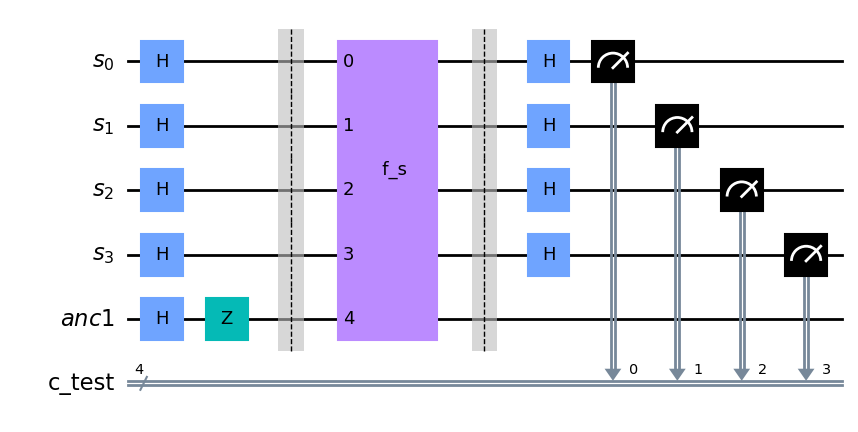
\includegraphics[width=0.8\textwidth]{TFG/imagenes/BV_circuito.png}
    \caption{Circuito, algoritmo BV para s de longitud 4} 
 \end{figure}

 Detallemos brevemente los elementos principales de este circuito:
 \begin{itemize}
     \item \textbf{Qubits}: Se representan en las primeras lineas, cada uno en una línea distinta. El circuito de la figura 2.1 se compone de 5 qubits. Entre ellos vemos un qubit llamado anc1, que es un qubit ancilla, auxiliar. Muchas veces este qubit extra almacenará el resultado de las operaciones, ya que nunca deberíamos modificar los datos originales. Se debe seguir el siguiente esquema: \newline
     
     \begin{center}$\Qcircuit @C=1em @R=.7em {\lstick{|x\rangle}&  \multigate{1}{U_{f}} &\qw & \rstick{|x\rangle}\\ \lstick{|y\rangle} &\ghost{U_{f}} & \qw & \rstick{|y \oplus f(x)\rangle}}$ \end{center}
     
     \item \textbf{Bits clásicos}: Se representan en la ultima fila, todos juntos. Podemos ver el número, en este caso 4, que nos indica el número de bits clásicos que tenemos.
     \item \textbf{Puertas para un qubit}: Podemos observar puertas ya conocidas como Hadamar, Z o la medición que vemos como cae hacia el cable de bits clásicos indicando en que bit se registra la medición.
     \item \textbf{Puerta $f_{s}$}: Como ya mencionamos anteriormente puede haber puertas que se apliquen a varios qubits, en este caso tenemos la puerta, o bloque, que replica la función del problema de Bernstein-Vazirani. Dentro de esta puerta tenemos puertas más pequeñas como las presentadas anteriormente en este mismo apartado. En particular, $f_{s}$ tiene puertas CNOT. En diversos algoritmos, se representa esta puerta como un bloque debido a que la podemos entender como un oráculo, del que no sabemos como funciona internamente.
     \item \textbf{Barreras}: Nos sirven como apoyo para visualizar el algoritmo y poder separar en secciones.
 \end{itemize}

 Para producir este circuito se puede hacer de distintas maneras, ya sea programando en python con apoyo de qiskit o directamente en IBM es posible poner las cajas de los operadores en los qubits que nos interesan.
 
\subsection{Simulaciones y ruido} 
 Una vez que ya hemos visto las puertas que podemos usar en un circuito cuántico, así como un ejemplo del mismo, veamos una introducción a las distintas opciones para la ejecución, utilizaremos las dos siguientes: (qiskit, intro cuantica)
 
 \begin{itemize}
     \item \textbf{Simulación}, en nuestro caso con los simuladores de IBM. Esta posibilidad nos va a ofrecer una simulación teórica de lo que ocurre en nuestro circuito. Será ejecutado a través de un simulador de IBM y nos va a permitir obtener resultados con seguridad y sin ningún problema asociado de errores o ruido.
     \item \textbf{Ordenador cuántico}, utilizaremos los ordenadores de IBM. La tecnología para la creación de ordenadores cuánticos más fieles sigue avanzando. Esta intenta mitigar los errores que tiene cada operación, así como los errores relacionados con el ruido del entorno que influyen en el estado del sistema modificándolo. Cada ordenador tiene su propia estructura y sus estudios sobre los errores que se cometen en cada qubit, así como calibraciones. Se puede ver en la figura 2.2, los errores de cada qubit así como la estructura del ordenador. Qiskit analizará el circuito y lo adaptará a la arquitectura del sistema elegido para minimizar los errores.
 \end{itemize}

 Ambas opciones utilizan el mismo mecanismo, repiten el proceso tantas veces como les sea requerido y muestran la frecuencia acumulada de los resultados (mediciones) o directamente las probabilidades sobre el número total de ejecuciones.

 
 \begin{figure}[H]
    \centering
    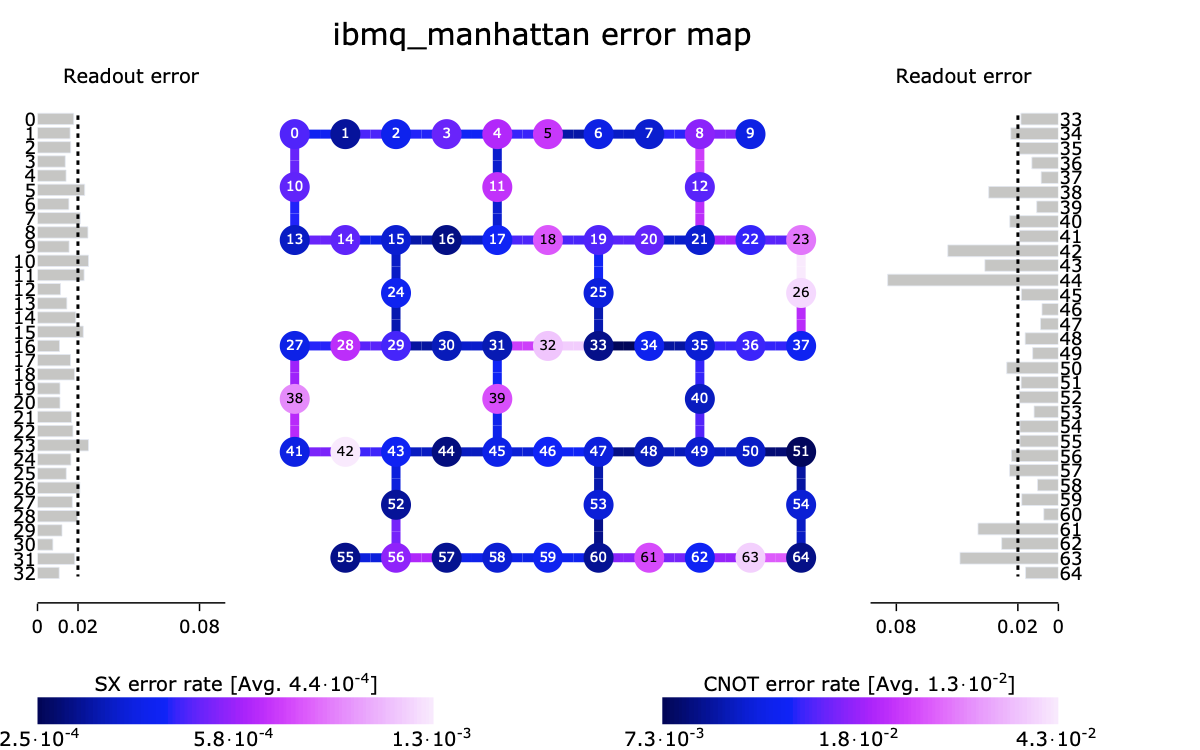
\includegraphics[width=\textwidth]{TFG/imagenes/system_error_manhattan.png}
    \caption{Mapa de errores del ibmq\_manhattan} 
 \end{figure}
 
 \vspace{5pt}
 
 Veamos un ejemplo para entender la diferencia de resultados de utilizar un opción u otra. Para ello vamos a usar los resultados del circuito presentado en la figura 2.1 del algoritmo de Bernstein-Vazirani que se presentará en el siguiente capítulo. Este algoritmo nos debería dar un resultado único, pero veamos lo que ocurre. \newline

 \begin{figure}[H]
    \centering
    \begin{subfigure}[H]{0.48\textwidth}
        \centering
        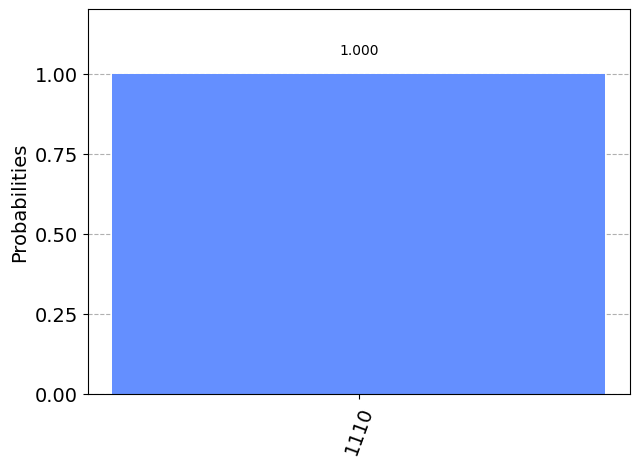
\includegraphics[width=\textwidth]{TFG/imagenes/BV_simulación.png}
        \caption{Simulación}
    \end{subfigure}
    \hfill
    \begin{subfigure}[H]{0.48\textwidth}
        \centering
        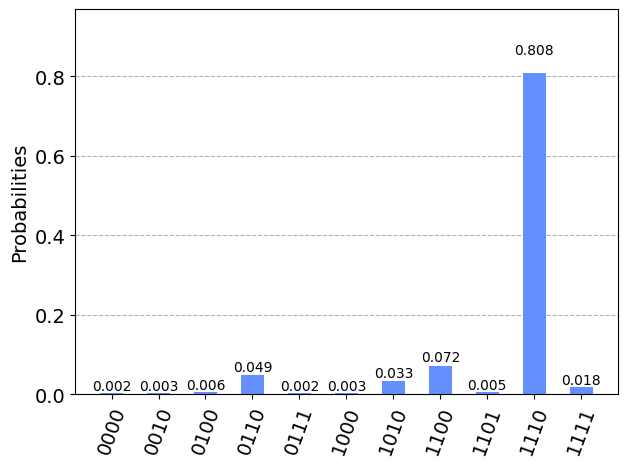
\includegraphics[width=\textwidth]{TFG/imagenes/BV_ruido.png}
        \caption{Sistema cuántico}
    \end{subfigure}
        \caption{Diferencias en resultados de ejecución del algoritmo de Bernstein-Vazirani}
 \end{figure}
\vspace{5pt}

Se puede observar en la figura 2.3 la diferencia entre la simulación teórica (a) y la ejecución con el sistema ibmq\_quito (b). Nuestra simulación nos ha dado únicamente el resultado querido, pero al ejecutarlo en sistema cuántico nos ha dado una variedad de resultados, aunque no todos los posibles. Si bien es cierto que el más probable, con suficiente diferencia, es idéntico al obtenido con la simulación. Cabe destacar de la figura 2.3.b que los de mayor probabilidad, una vez eliminada la solución, son aquellos en los cuales solo varía 1 dígito y por el contrario, el complementario binario no ha aparecido como resultado en todas las ejecuciones realizadas.

\section{Propiedades Metamórficas / Testing metamórfico}

Informalmente entendemos como propiedad metamórfica aquella que podemos derivar de forma lógica de una definición o especificación. Empecemos con un ejemplo para ponernos en situación, nos vamos a fijar en la función seno, $f(x)=sin(x)$.\newline

La definición que aprendemos cuando empezamos a ver trigonometría es que el seno es la proporción entre el cateto opuesto y la hipotenusa en un triángulo rectángulo. Teniendo esta imagen la cabeza es muy fácil darse cuenta que $sin(x)=sin(x + 2\pi)=sin(\pi-x)$. Estas son dos propiedades metamórficas de la función seno. \newline

Veamos ahora que es lo que consideramos formalmente una regla o propiedad metamórfica y como llegamos a los pasos de testing metamórfico: (Metamorfic testing paper)

\begin{itemize}
    \item \textbf{Relación metamórfica}, PM: Sea $f: X \rightarrow Y$ una función o algoritmo. Se considera que $\mathscr{R} \subseteq X^{n} \times Y^{n}$ es una \textbf{\textit{regla metamórfica}} si es una relación entre una secuencia de entrada $\langle x_{1},x_{2},...,x_{n}\rangle$ con $n>1$ y sus salidas correspondientes $\langle f(x_{1}),f(x_{2}),...,f(x_{n})\rangle$, la cual se puede deducir de forma lógica desde el algoritmo. Es decir, es una propiedad necesaria de f.
    \item \textbf{Entrada original/seguimiento}: Sea $\mathscr{R}$ una relación metamórfica y sea $\langle x_{1},x_{2},...,x_{k}\rangle$ la secuencia original con sus respectivos resultados. Denotaremos como \textbf{\textit{entrada original}}, source input, a   $\langle x_{1},x_{2},...,x_{k}\rangle$  los cuales son datos definidos o caracterizados, es decir, ya conocidos. A su vez, podemos generar $\langle x_{k+1},x_{k+2},...,x_{n}\rangle$, los cuales están construidos en base a la entrada original e incluso a la salida de esta. A esta secuencia la llamaremos \textbf{\textit{entrada de seguimiento}}, o en inglés follow-up input.
    \item \textbf{Grupo metamórfico de entrada}: Llamaremos \textbf{\textit{grupo metamórfico de entrada}} a la secuencia definida por la entrada original y la de seguimiento, es decir, $\langle x_{1},x_{2},...,x_{k},x_{k+1},...,x_{n}\rangle$.
    \item \textbf{Testing metamórfico}, TM: Sea $f$ la función o algoritmo objetivo, $P$ una implementación de $f$ y $\mathscr{R}$ una regla metamórfica de $f$. Para realizar \textbf{\textit{testing metamórfico}} sobre $P$ seguiremos los siguiente pasos:
    \begin{itemize}
        \item Definimos $\mathscr{R}'$ reemplazando $f$ por $P$ en $\mathscr{H}$.
        \item Dado una entrada original, generamos sus salidas según $P$, construimos a partir de estos, los casos de seguimiento $\langle x_{k+1},...,x_{n}\rangle$, y obtenemos $\langle P(x_{k+1}),...,P(x_{n})\rangle$.
        \item Estudiamos los resultados obtenidos respecto a $\mathscr{R}'$. Si no es satisfacible entonces diremos que $P$ no es correcto.
    \end{itemize}
\end{itemize}

La estrategia presentada anteriormente para TM, será la que se siga en la implementación de las propiedades que se obtendrán a lo largo de este documento. \newline

Para finalizar con esta introducción vamos a revisar brevemente un par de ventajas y retos que presenta el camino que estamos tomando para probar la corrección, o más bien la no corrección, de un algoritmo. \newline

\textbf{Ventajas}:
\begin{itemize}
    \item \textbf{Simplicidad}. El concepto e interpretación de una PM es bastante simple en comparación con otros conceptos que se utilizan dentro del campo del testing. Se ha visto en estudios, que incluso gente con poca experiencia, podrían utilizar estas técnicas en relativamente poco tiempo de forma efectiva.(ref 55,73 del paper de testing)
    \item \textbf{Facilidad en la implementación}. Si partimos de la ventaja anterior como es la simplicidad de la definición, podemos continuar que la implementación de este test es prácticamente seguir los pasos explicados en la definición de TM (link a la definicion).
\end{itemize}

\vspace{10pt}

\textbf{Retos}:
\begin{itemize}
    \item \textbf{Generación efectiva de los grupos metamórficos de entrada}. Aun se sigue estudiando que garantías tenemos en la efectividad que puede tener la elección del grupo metamórfico de entrada en la demostración de la corrección de un algoritmo y en particular, la forma en la que obtenemos nuestra entrada original, ya que la entrada de seguimiento la generamos a partir de esta. Al fin y al cabo nuestro objetivo es maximizar la identificación de errores o defectos en $P$.
    \item \textbf{Estructura del TM}. Debido a la juventud de este tipo de testing y la gran variedad de PM, aun no hay un acuerdo sobre una estructura definida y formal que nos proporcione seguridad en nuestra pruebas y englobe a todas las posibilidades que tenemos dentro de las PM. Aunque, si bien es cierto, ya ha ayudado a identificar diversos errores en sistemas muy estudiados con otros métodos de testing, como por ejemplo los compiladores GCC y LLVM de C, en los cuales encontró más de 100 defectos (\textit{faults}). (ref 50,51,78)
\end{itemize}

Los retos de TM pueden ser una buena base para todo el trabajo futuro que se puede realizar en este campo y las posibilidades que este nos puede ofrecer. Trataremos en más profundidad estás posibilidades en el apartado 5.2 de posibles trabajos futuros (link)



